\begin{figure}[H]
\centering
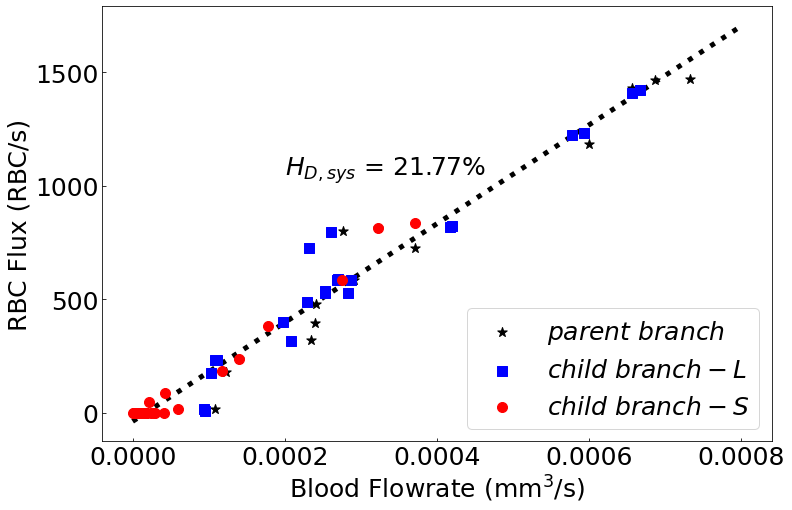
\includegraphics[width=0.95\textwidth]{images/SystemHaematocrit.png}
\caption{\textit{RBC flux against Blood flow rate including best-fit line. The "L"/"S" indicate the relatively larger (blue squares) and smaller (red circles) child branches in each diverging bifurcation respectively.} \label{SystemHaematocrit}}
\end{figure}
